\chapter{Implementation of the mem-HNN}

\section{Zielsetzung und Forschungsmethodik}
Upon establishing the precise research methodology, this chapter delves into the practical application of the previously mentioned methods.
First, the analysis phase of the \ac{DSR} process is executed with the goal to establish a model of the research plan 
which the requirements and framework conditions of the \ac{IT}-solution can be derived from. 
Next, the practical implementation is performed during the iterative design phase and uses the method of prototyping.
In the end of the design phase is a functional \ac{IT}-artifact, which fulfills the set requirements.
The evaluation phase in this chapter uses the method of simulation to answer the second part of the research question; to see how efficient 
the \ac{mem-HNN} can utilize the AI-model in terms of throughput and energy usage.

\section{Analysis phase}
\subsection{General conditions}
The first phase of the \ac{DSR}-cycle has the goal of specifying the objective and establishing an according research outline and the requirements of the artifact.
Additionally, the research outline should be visualized as a model of the overall solution concept.\footcite[cf.][278-279]{oesterleKonsortialforschung2010}
The objective of the practical part is already specified in chapter 3.1.
The underlying motivation hereby is to research if the known proof of concepts are feasible on the complete \ac{mem-HNN}
and evaluate if that brings an actual acceleration, which is equivalent to answering the research question of this thesis. 
This is tested by implementing the concept in software that is also part of the ASIC design process.\footnote{cf.\cite{raoUltimateGuideASIC}, p. 1; cf.\cite{ASICDesignFlow}, p. 1}

The implementaton is executed in the programming language Python since it offers a variety of third party libraries that are useful 
for machine learning that are state of the art, like pytorch, scikit learn etc..\footcite[cf.][306-307]{DiscreteContinuousModels}
Furthermore, scikit learn is chosen as machine learning library since it is one of the industry standards for classical machine learning, has a broad variety of features in terms of \ac{RBM}s
and has a lower learning curve compared with e.g. Tensorflow.\footcite[cf.][5-6]{raschkaMachineLearningPython2020}

It should also be clarified that the hardware, which the analog \ac{mem-HNN}-accelerator consists of, is implemented in software. 
This design decision is made out of time constraints of this thesis and part of the ASIC design process before buildng an actual accelerator. 
Nonetheless, the complete hardware is realizable in software without taking compromisses within their functionality.
The simulation data gathered later on is close to the real energy efficiency and throughput.\footcite[cf.][3-4]{hizzaniMemristorbasedHardwareAlgorithms2023} 


Lastly, the energy model used in the simulation can, depending on a specific input, calculate the amount of energy required from the hardware to perform computations.
This energy model is developed by HPE and the Forschungszentrum Jülich.
The explanation for this model is out of scope for this thesis but core parameters are explained to understand the data generation for the energy values.
A seperate paper will be published about the energy model in the near future but kindly for this thesis the model can be used in advance.

\subsection{Requirements}

In order to set requirements for the IT-artifact an ideal overall solution architecture is of importance. 
Hence, a complete solution is modelled, which surpasses both proof of concepts introduced in 2.4.4.
It shows the components required for an acceleration of a \ac{BM} in hardware with the statistical sampling performed by an Hopfield Network, which was never done and tested before.
Furthermore, the following figure\ref{Overall architecture} contains the interaction between the digital computer and the analog mem-HNN Accelerator with five different steps. 
\begin{figure}[H]
    \centering
    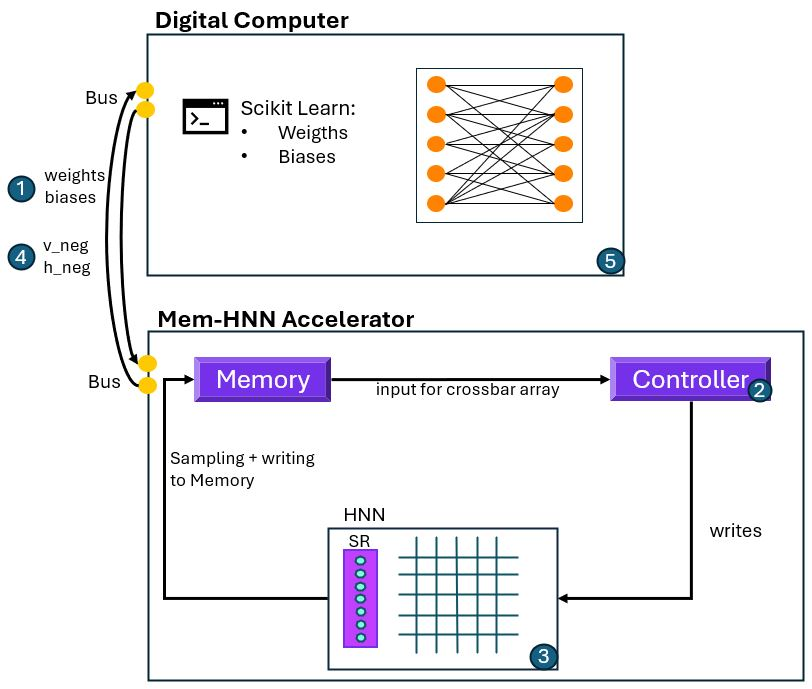
\includegraphics[width=0.80\linewidth]{graphics/Analysemodell.JPG}
    \caption{proposed solution architecture}
    \label{Overall architecture}
\end{figure}
\textbf{1.} contains the initialization of the neural network. 
Hence, the weights and biases are assigned and the structure is build.

\textbf{2.} starts with the transfer of the weigths and biases to the \ac{mem-HNN} accelerator via a bus-system. 
The local memory saves the data and forwards them to the controller. 
The controller is able to programm the memristors in the crossbar array, communicates with the computer and sets a counter and reset for the amount of sampling steps. 

\textbf{3.} is the Hopfield Neural Network (HNN), which contains the memristor crossbar array and the state register (SR).
The state register includes the current neuron configuration.\footcite[cf.][18]{caiHarnessingIntrinsicNoise2019}
For each of the neurons a \ac{TIA} and comparator are required in the hardware.
Furthermore, the state register can lock und unlock specific neurons, so that it is possible to update neurons synchronously.
This enables the possibility of the promissing N/2 update strategy.

\textbf{4.} After iterating over steps two and three multiple times until enough sampling are executed the, all the configurations
of the visible neurons \(v_{neg}\) and the  hidden neurons \(h_{neg}\) are transferred from the controller via the bus-system to
the digital computer. 

\textbf{5.} contains the update of the weights and biases. 
Furthermore, the model can be evaluated in its performance in terms of chosen metrics like prediction accuracy or the negative likelihood etc..
In this case a logistic regression is used for the classification task and the \ac{RBM} is used for the trainng of the neural network. 
After the evaluation the iteration is completed and the new weghts and biases can be transmitted for the following training iteration.

Since such chips do not yet exist, the objective is to construct a simulator pipeline that integrates these individual steps into a simulator, effectively replicating this hardware platform.
Only the bus system, the memory and the controller are not mappable since the local machine already has the hardware.
With this underlying model deriving the requirements is the next step in establishing the research outline.
The aim of generating requirements is to generate good quality, not perfect, requirements that offers an acceptable level of risk to start the project.\footcite[cf.][11]{ebertSystematischesRequirementsEngineering2008}
Hence, these requirements need to cover the functions of the \ac{mem-HNN}, which then must be implemented by the respective software components.
Despite this, requirements may evolve over time and occasionally require adjustments when outcomes differ from initial expectations.
As a result, the analysis of the model in conjunction with the reasearch question and under thought of the defined objective, the following requirements for the software emerged:

\textbf{Digital Computer}
\begin{itemize}
    \item Defining a \ac{RBM}
    \item Utilization of any training data
    \item Training a \ac{RBM}
    \item Establishing a pipeline for the classification
    \item Possibility of conventional sampling algorithms: gibbs sampling and metropolis hasting
    \item Setting individual parameters: sampling steps, training iterations 
\end{itemize}
\textbf{Simulated Mem-HNN Accelerator}
\begin{itemize}
    \item Using any \ac{RBM} as input
    \item Correctly using the Hopfield Network update algorithm
    \item Return sampled output of the neuron configurations 
    \item Correctly using the Hopfield Neural Network as sampling method 
    \item Possibility to use N/2 half updating method instead of asynchronously update of states
    \item Component for measuring the parameters required for evaluation: Speed (throughput) and energy consumption
\end{itemize}
Fruthermore, the python program should be split logically into the different modules and components to enable well structured code. 
With set requirements it is now possible to begin the iterative design and evaluation cycle with focusing on some requirements per iteration.

\section{First Design and Evaluation phase}

This \textbf{Design phase} includes the establishment of a prototype that impelments all requirements of the digital computer.
The first step is to perform in prototyping is the systemic analysis of the desired prototype used for categorization.
Hereby, the type of prototype(1) is computational, the fidelity level(2) is high since all functionalities should be modelled and be close to reality. 
Furthermore, the complexity(3) is considered sub since not every single hardware component can be modelled in software. 
Last but not least, the scale(4) stays the same the number of iterations(5) are multiple that are executed sequential in order to train and interfer the \ac{RBM}.
Well-suited for the implementation of a \ac{RBM} in python are machine learning libraries. 
In this case scikit learn is chosen since it is one of the industry standards for classical machine learning, has a broad variety of features in terms of \ac{RBM}s
and has a lower learning curve compared with e.g. Tensorflow.\footcite[cf.][5-6]{raschkaMachineLearningPython2020}
The implementation of the \ac{RBM} is inspired by the example of the official scikit learn documentation.\footcite[cf.][1]{RestrictedBoltzmannMachine}
Here, the RBM model is modelled as the feature extractor in combination with a logistic regression classifier.

\begin{lstlisting}
    logistic = linear_model.LogisticRegression(solver="newton-cg", tol=1)
    rbm = BernoulliRBM(random_state=0, verbose=True)
\end{lstlisting}
Scikit learn offers a variety of datasets that are already in a polished format, ready to use. 
The decision is to use a classification workload of handrwritten digits.
This load digits dataset is similar to the well known MNIST dataset but has a smaller resolution of 8x8 pixels and features around 1800 samples that can be categorized in 10 classes (integers 0-9).\footcite[cf.][1]{SklearnDatasetsLoad_digits}
The dataset can be changed as desired with for example a breast cancer classification workload; in general all datasets that have two states like the activation of neurons in the neural network are compatible.
In this case additionally a nudging of the data is happening to create more samples, by a factor of five, and to bring more complexity. 
The dataset was divided into 80\% training data and 20\% test data.

Parameters like the learning rate, iterations, size of the hidden layer need to be set. 
With having a look in the literature and through testing a learning rate of \(0.2\), 10 training epochs with 72 iterations in one epoch, and an hidden layer of 100 neurons is chosen.
The size of the visible layer is automatically recognized by scikit learn and set to 64 since the resolution 8x8 requires that amount to pricess the input.

The training of the \ac{RBM} works with the 
\texttt{.fit} method and for the possibility to select the preferred sampling algorithm 
an additional parameter \texttt{sampling\_method} is added. 
\begin{lstlisting}
    if sampling_method == SamplingMethod.GIBBS:
    v_neg = self._sample_visibles(self.h_samples_, rng)
    h_neg = self._mean_hiddens(v_neg)
    
    elif sampling_method == SamplingMethod.METROPOLIS_HASTING:
    h_neg,v_neg=mcmc_sample(10000,len(self.components_))
\end{lstlisting}
This process includes radically changing the \texttt{\_rbm.py} file in the scikit learn library within the \texttt{neural\_network} folder.
The predefined sampling method is gibbs sampling and there is no option to access metropolis hasting within the basic library. 
Therefore, the metropolis hasting alhorithm, explained in 2.2.3 needs to be manually implemented.
The according adjustments are inspired and modified by the code availability of a paper, which was published in Nature Communiations.\footcite[cf.][11-12]{bohmNoiseinjectedAnalogIsing2022}
Another promising approach to evaluate the performance of the neural network is to predict on the test data after every iteration.
A complete code overview of the metropolis hastings sampling algorithm can be found in the \texttt{mcmc2.py} file with all
the adjusted methods for the training of the \ac{RBM} are made in \texttt{\_rbm.py}, while the overall execution takes place in the \texttt{playground.py}.

Hence, the possibility of different sampling methods are possible and the training of the \ac{RBM} is possible.
To evaluate the results and functionalities the \textbf{Evaluation phase} in this iteration validates the functionalities through a training of the \ac{RBM} with each sampling method and extract their prediction accuracy 
and negative likelihood for each iteration. Following figure\ref{CD_baselines} shows the training results using the gibbs sampling approach. 

\begin{figure}[H]
    \centering
    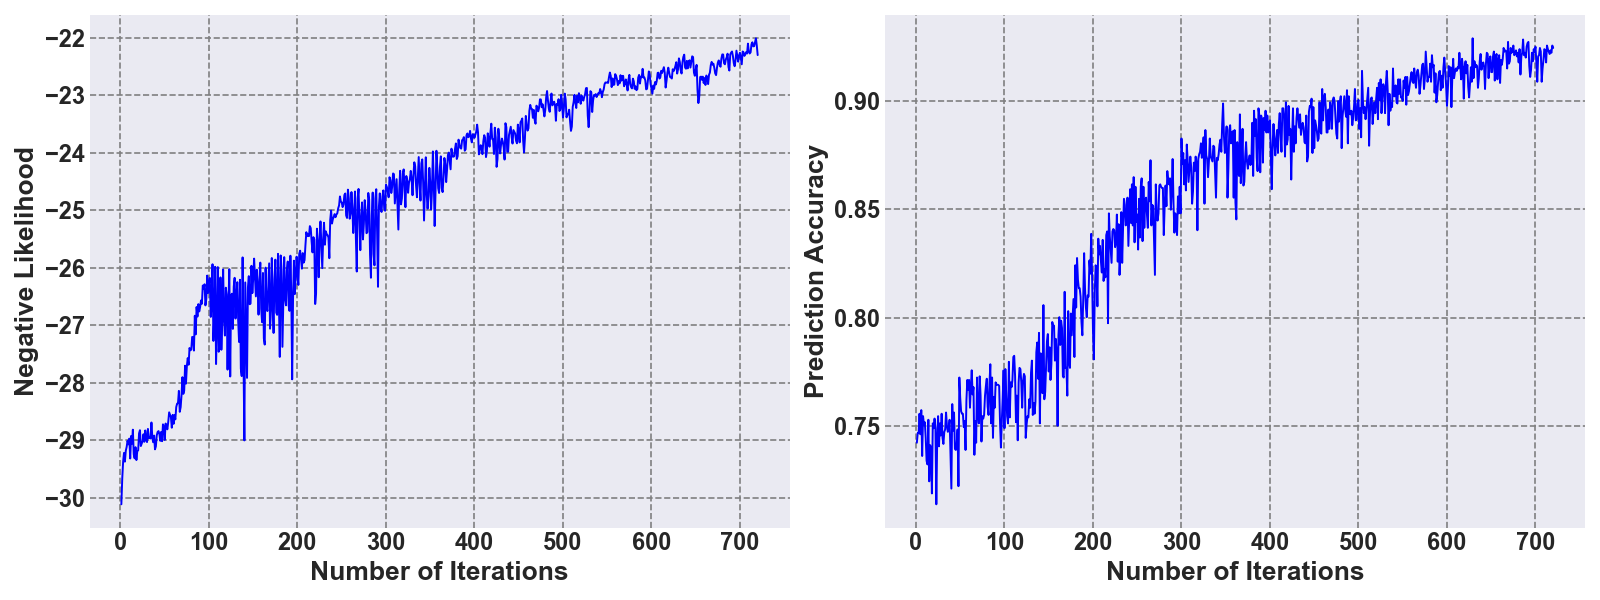
\includegraphics[width=1\linewidth]{graphics/CD_combined_plot.png}
    \caption{Gibbs sampling baselines}
    \label{CD_baselines}
\end{figure}
The right plot clearly shows that the initial prediction accuracy starts at 75\%, akin to that of a linear regression model.
This suggests that without training a linear regression alone could account for this level of accuracy when an untrained \ac{RBM} is included in the pipeline.
Data points are colected after every iteration across the span of 720 iterations. 
It is noteworthy that after 650 iterations the accuracy tagnated and had a maximum prediction accuracy
of 92.29\%. 

In the left plot picturing the negative likelihood, which is a measure of how well a statistical model represents the observed data.
When training a model the aim is to minimize the negative log-likelihood, which means that the model maximizes the probability of generating the observed data.
Hence, it is visible that in the beginning the model learns more rapidly and in steadily grows its knowledge with some smaller break-ins at the end.
The best value is a negative likelihood of -22.01.
\begin{figure}[H]
    \centering
    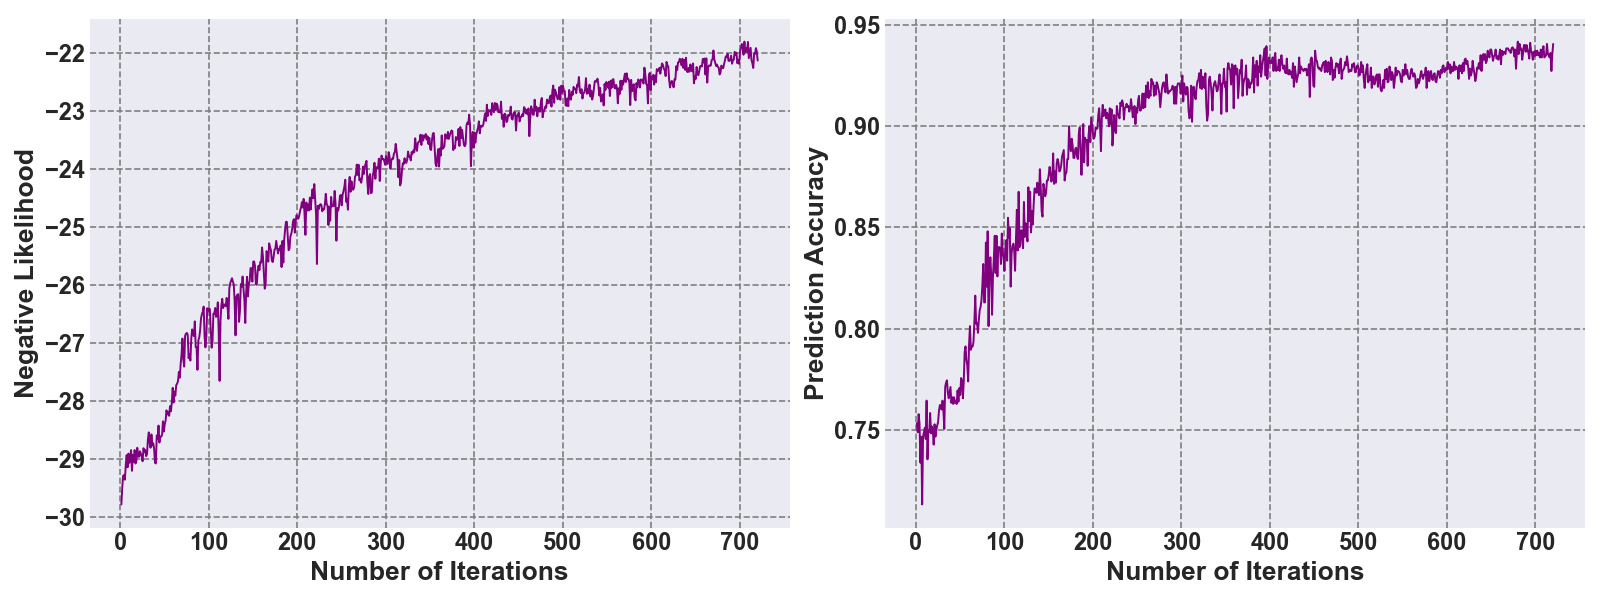
\includegraphics[width=1\linewidth]{graphics/metropolis_combined_plot.png}
    \caption{Metropolis sampling baselines}
    \label{metropolis_baselines}
\end{figure}
In contrast, the figure\ref{metropolis_baselines} used the sampling algorithm of metropolis hasting to train the \ac{RBM}.
Noteworthy is that the prediction accuracy in the right plot has a faster increase in the beginning but already starts to stagnate at around 400 iterations. 
Here, the maximum prediction accuracy already returned 94.15\%. 
The negative likelohood is also growing faster than in gibbs sampling and has less spikes in the beginning showing a more continuously learning rate.
Here, the best negative likelihood value is -21.80.
The gathered data can later on be used as baseline against the desired new updating mehtod of sampling with a Hopfield Network.
As a result, with each sampling method successfully undergoing a training, all the functionalities can be proven right and the prototype can be passed 
into the next design iteration.


\section{Second Design and Evaluation phase}

This \textbf{design phase} iteration lays its focus on the implementation of correctly using the Hopfield Network update algorithm. 
Following subfunctionalities need to be established: imitating the \ac{RBM} activation function, drawing random neurons to update,
correct injection of the gaussian noise scale, calculating the weighted sum,
comparing the weighted sum + bias + noise agaisnt the threshold and saving the new neuron configuration.
Hence, this iteration is accessing new ground since the implementation of the simulator pipline is not validated yet. 

First, a new \texttt{\_hopfield\_network\_v1.py} is created that aims to establish a noisy Hopfield Network with a single neuron 
and meassure its activation function.
Like mentioned in 2.4.4, a Hopfield Network has a binary activation function that needs to be made compatible with the sigmoid activation function of the \ac{RBM}.
The Hopfield Network is initialized with a size of just one neuron and an sampling iteration counter of \(1500\) iterations with a thermalization of \(100\) sampling steps before 
the neuron is updated.
A thermalization is used so that the internal network can get into a flow and do some sampling steps to be statistical independent in order to have un unbiased sampling.
The threshold as defined in the Hopfield Network update formula is \(0\). 
As experimented the update formula for implementation of the Hopfield Network looks the following:

\begin{lstlisting}
    for x in range(self.iterations_per_theta):
                    
        self.neuron_index = np.random.randint(0, self.size) #pick a random neuron in the network
        # Calculate the weighted sum for the neuron, excluding its own state
        weighted_sum = sum(self.weights[self.neuron_index][j] * self.configuration[j] for j in range(len(self.configuration)) if j != self.neuron_index)

        self.new_configuration = deepcopy(self.configuration)   #copying the old configuration to create a new one and update it
        if (weighted_sum + self.bias + np.random.normal(0, scale=1.75)) >= self.threshold_theta:          
            self.new_configuration[self.neuron_index] = 1
        else:
            self.new_configuration[self.neuron_index] = 0
            
        self.configuration = deepcopy(self.new_configuration)   #Cloning current configuration and updating the cloned version to the new configuration after comparing with threshold

        if x >= self.thermalization:  
            self.summedConfigurations = self.sum_configurations(self.summedConfigurations, self.new_configuration)    
            self.iterationcounter += 1
        
    self.activationProbabilityPerNeuronDict[self.bias] = self.divide_array_elements(self.summedConfigurations, self.iterationcounter)
    self.bias += 0.025
\end{lstlisting}
In the beginnig a random neuron is drawn to be updated, which currently everytime is neuron number one because the network size is one. 
This allows to meassure the activation probability and fast iteration time with a clear result on how the network behaves. 
Calculating the weighted sum can be seen as the core of the update formula and is done first.
Afterwards to compare against the threshold an bias is added.
The value of the bias ranges from \(-6; 6\) in step sizes of \(0.025\). After completing all samplin iterations beginning with \(-6\) the step size is added to that value until all iterations are made.
This is sufficient for the neuron activation function of an ordinary Hopfield Network and results in the binary step. 
The resulting activation function is obtained by summing all configurations within a single bias configuration.
In a next step, the configurations counted are divided by the number of total sampling iterations within the bias configuration (in this case 1500 iterations).
That following figure \ref{Noisy_acitivation_function_bad} \textbf{evaluates} the resulting activation probability of the single neurons. 
\begin{figure}[H]
    \centering
    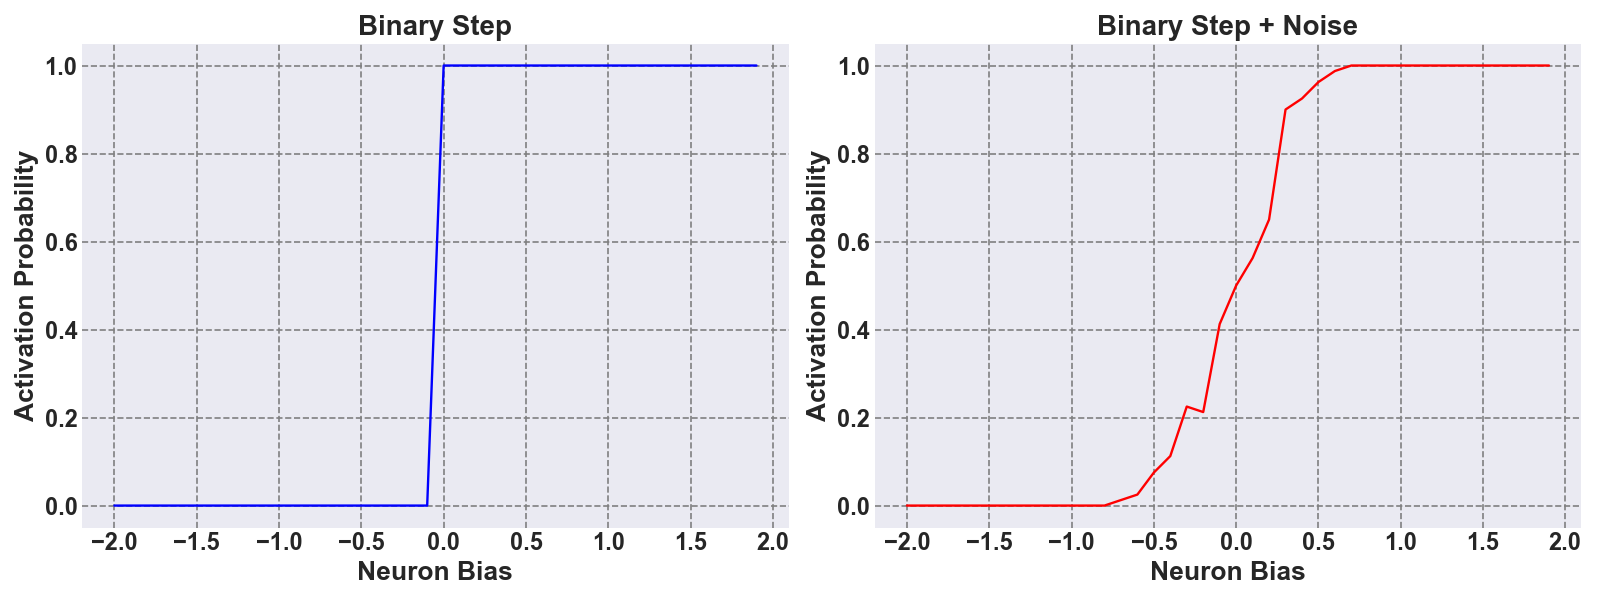
\includegraphics[width=1\linewidth]{graphics/combined_noise_activation_plots.png}
    \caption{Modification of the binary step activation function of the Hopfield Network}
    \label{Noisy_acitivation_function_bad}
\end{figure}
In the left plot, visualized in blue, the activation probability of the neuron is shown without adding noise to the plot. 
The behaviour is like sme would expect it; once the bias reaches 0 the neuron is activated all the time.
Far more interesting is the red plot on the right side, which introduces some noise into the binary step function, bringing it closer to the logistic sigmoid activation function used in the \ac{RBM}.
To achieve this behavior, injecting noise through a Gaussian normal distribution can modify the activation function, making it compatible with the sigmoid function.\footnote{cf.\cite{bohmNoiseinjectedAnalogIsing2022}, p. 1-2; cf.\cite{mahmoodiVersatileStochasticDot2019}, p. 2}"
Technically this is performed by adding \texttt{np.random.normal(0, scale=1.75)} to the weighted sum and the bias, with 0 beeing the mean of the distribuion and the scale representing the standard deviation. 
Hereby, it is important to find a standard deviation that is very close to the true activation probability is important, otherwise the training of the RBM would not work.
In addition to that, the standard deviation changes with neuron size and needs to be readjusted if changes are made to the networks structure.
So what is visible in the right plot that the sigmoid function is not correctly imitated but proves that the
Concluding from this the sigmoid function is not achieved and the trainig of an \ac{RBM} probably fails. 
Therefore, to completely evaluate and ensure that the injected noise fits to the logistic sigmoid function, the function itself is plotted 
too, to have a visual comparision. Afterwards, finding the correct standard deviation is the goal. 
In following figure\ref{Noisy_acitivation_function_good} the compatibility is verifired:
\begin{figure}[H]
    \centering
    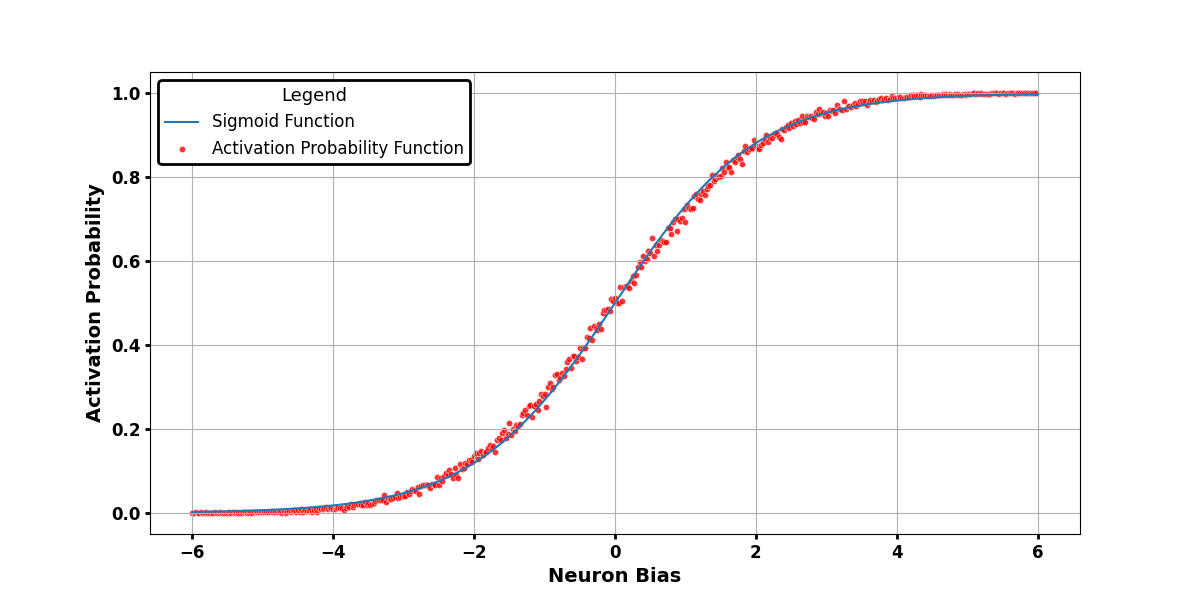
\includegraphics[width=1\linewidth]{graphics/Noisy_HNN_2.png}
    \caption{Noisy activation function of the Hopfield Network imitating the \ac{RBM}}
    \label{Noisy_acitivation_function_good}
\end{figure}


\section{Third Design and Evaluation phase}

Using any \ac{RBM} as input
Return sampled output of the neuron configurations 
Correctly using the Hopfield Neural Network as sampling method 


\section{Fourth Design and Evaluation phase}

Possibility to use N/2 half updating method instead of asynchronously update of states
% Component for measuring the parameters required for evaluation: Speed (throughput) and energy consumption

\section{Final Evaluation phase}

Simulation: Component measuring the parameters required for evaluation: Speed (throughput) and energy consumption


-Testen der Aktivierungsfunktion, wenn ich ein Neuron trainiere und dann Mitteln 
- Von vornerein auf Netzwerk Basis arbeiten mit mehren Neuron, jedoch für 1 Neuron testen



Hopfield Netzwerk aktivierungsfunktion der Updating methode

-> Konzeptionell Art des Updates mit keiner Temperatur wie bei MCMC 
Unterschied von MCMC zu Hopfield Netzwerk -> Zufällige Konfiguration und minimale Energie finden. Jedoch hat ein Hopfield
Netzwerk keine Temperatur 

-> Starte zufällige Konfiguration
-> Wähle ein Neuron aus und Berechne Summe und addiere mit Bias, 
-> Update wenn thresshold überschritten 1 und dann auf 0 
-> Speichern der neuen Konfuguration 
-> Starte iteration von gespeicherter Konfiguration 
-> Am Ende habe ich 10000 Vektoren (Die Konfigurationen) -> V1 Neuron wurde so und so oft aktiviert und ich muss average
über das neuron und habe dadurch die Aktivierungswarscheinlichkeit.

-Aktivierungsfunktion einfügen (Binary Step und verfleich zu sigmoid von Abb.4)



\section{Evaluation phase}

Aufbau der Simulator Pipeline
KI-Bibliothek Scikit-Learn
Evaluationsphase

To integrate simulation into the DSR concept ... 
The desired result of the prototyping is completing the \ac{DSR} design phase and with a simulation the result should be verified.
The input is the finished prototype, that mirrors the functionalities of the \ac{ASIC} on a high level.
